\documentclass[aspectratio=169,11pt]{beamer}
\usetheme{default}
\usefonttheme{professionalfonts}
\usepackage{amsmath,amssymb,graphicx,booktabs}
\setbeamertemplate{navigation symbols}{}
\setbeamertemplate{footline}[frame number]
\setbeamerfont{frametitle}{series=\bfseries}
\setbeamercolor{frametitle}{fg=black}
\definecolor{acc}{HTML}{1F5FAD}
\setbeamercolor{itemize item}{fg=acc}
\setbeamercolor{enumerate item}{fg=acc}
\newcommand{\hl}[1]{\textcolor{acc}{\textbf{#1}}}

\begin{document}

% ===================== PROBLEM (2 min) =====================

\begin{frame}{Problem: can a complex model time the market?}
\begin{columns}[T]
\begin{column}{0.49\textwidth}
\footnotesize
\hl{Task.} Predict next month's excess return of the CRSP value-weighted index from the 15 Goyal--Welch predictors $G_t$ (dp, dy, ep, de, svar, b/m, ntis, tbl, lty, ltr, tms, dfy, dfr, infl, lagged return), 1926--2020.

\smallskip
\hl{Consensus} (Goyal \& Welch, 2008): out of sample these predictors do not beat the historical mean $\Rightarrow$ use simple models.

\smallskip
\hl{Puzzle.} ML models have $P\gg T$. Textbook statistics: overfitting. KMZ: complexity is a \emph{virtue}.

\smallskip
\hl{Data} (\texttt{voc\_data.py}, Sec.~V.A):
\begin{itemize}
\item returns $/$ trailing 12-month uncentered std
\item predictors $/$ expanding std, $\ge 36$ months
\item only past information $\Rightarrow$ sample starts in 1930
\end{itemize}
\end{column}
\begin{column}{0.49\textwidth}
\footnotesize
\hl{Model} (eqs.~1--3): unknown $f$ approximated by $P$ nonlinear signals
\[R_{t+1}=f(G_t)+\varepsilon_{t+1}\approx\sum_{i=1}^{P}S_{i,t}\,\beta_i+\varepsilon_{t+1}\]

\hl{Timing strategy} (eq.~6): position $=$ forecast
\[\pi_t=S_t'\hat\beta,\qquad R^{\pi}_{t+1}=\pi_t\,R_{t+1}\]

\hl{Evaluation} (eq.~5): economic value, not only accuracy
\[SR=\frac{E[R^{\pi}_{t+1}]}{\sqrt{E[(R^{\pi}_{t+1})^2]}}\]
\end{column}
\end{columns}
\end{frame}

\begin{frame}{Problem: why a bad $R^2$ can still pay}
\begin{columns}[T]
\begin{column}{0.54\textwidth}
\footnotesize
\hl{Prop.~1} (infinite sample, true $\beta$ known):
\[SR\;\to\;\frac{1}{\sqrt{3+(b_*\psi_{*,1})^{-1}}}\;<\;\sqrt{1/3}\approx0.58\]
Even the infeasible strategy has a modest ceiling.

\medskip
\hl{MSE decomposition} (eq.~8):
\[MSE(\hat\beta)=E[R^2_{t+1}]-2\underbrace{E[\hat\pi_tR_{t+1}]}_{\text{timing exp.\ return}}+\underbrace{E[\hat\pi_t^{\,2}]}_{\text{timing leverage}}\]
Large, noisy positions ruin MSE and $R^2$, yet the expected return of the strategy can stay positive.\\
$\Rightarrow$ negative $R^2\neq$ no economic value.
\end{column}
\begin{column}{0.44\textwidth}
\footnotesize
\hl{The claim} (Fig.~7, Table~I):
\begin{itemize}
\setlength{\itemsep}{4pt}
\item $P=12{,}000$ random Fourier features
\item $T=12$ months of training data, $c=P/T=1{,}000$
\item ridge $z=10^3$
\item out-of-sample $SR=\mathbf{0.47}$, 1930--2020
\item more complexity $\Rightarrow$ higher return and Sharpe
\end{itemize}

\medskip
\hl{Our data check:} same setting, 5 seeds $\Rightarrow SR\approx0.49$.
\end{column}
\end{columns}
\end{frame}

% ===================== CRITIQUE (3 min) =====================

\begin{frame}{Critique 1--2: momentum and a simple benchmark}
\begin{columns}[T]
\begin{column}{0.52\textwidth}
\footnotesize
\hl{Kernel view} (Nagel, 2025): with $P\gg T$ the forecast is a weighted average of the last 12 returns
\[\hat R_{t+1}\approx\sum_{s=t-12}^{t-1}w(G_t,G_s)\,R_{s+1}\]
Persistent $G$ $\Rightarrow$ recent months most similar $\Rightarrow$ volatility-timed time-series momentum.
\begin{itemize}
\item Nagel: vol-timed momentum IR 0.39 vs RFF 0.26; on simulated reversals RFF still bets on momentum and loses
\item Elmore \& Strauss (2025): forecasts 97.5\% correlated with past 12-month return
\item Cartea \& Shi (2025): flip the sign of returns $\Rightarrow$ the ``virtue'' reverses
\item KMZ, p.~499: acknowledge the link, report alpha over TSMOM
\end{itemize}
\end{column}
\begin{column}{0.46\textwidth}
\footnotesize
\hl{The paper's own Table I} ($z=10^3$, Sharpe):

\smallskip
\centering
\begin{tabular}{lcc}
\toprule
$T$ & Linear, $P=15$ & RFF, $P=12{,}000$\\
\midrule
12  & 0.46 & 0.47\\
60  & 0.44 & 0.42\\
120 & \textbf{0.49} & 0.41\\
\bottomrule
\end{tabular}

\raggedright
\medskip
Shrinkage, not 12{,}000 features, does most of the work.

\smallskip
\hl{Buncic (2025, rev.\ 2026):} implementation choices handicap simple models; standard linear models reach Sharpe ratios up to 40\% higher.

\smallskip
{\scriptsize In fairness: KMZ report IR 0.26 ($t=2.5$) of RFF over the linear model at $T=12$.}
\end{column}
\end{columns}
\end{frame}

\begin{frame}{Critique 3: how could this be overfit?}
\footnotesize
\begin{enumerate}
\setlength{\itemsep}{5pt}
\item \hl{$\gamma=2$ is a choice.} Paper: ``insensitive''. Our rerun: $\gamma=0.5,1,2,4\Rightarrow SR=0.27,\,0.36,\,\mathbf{0.49},\,0.35$
\item \hl{$T=12$ window.} Short window $+$ persistent predictors $=$ momentum by construction; RFF Sharpe falls to 0.42 / 0.41 at $T=60$ / 120
\item \hl{Standardization.} 12-month uncentered vol for returns, expanding std for predictors, 36-month burn-in: each step is a free choice
\item \hl{Shrinkage grid.} Headline $z=10^3$ is the top of $\log_{10}z\in[-3,3]$; no out-of-sample rule for choosing $z$
\item \hl{One sample.} US, 1930--2020; returns halve after 1975 (p.~499). Our rerun: $SR$ 0.57 before, 0.42 after
\item \hl{Data timing.} Inflation for month $t$ is published mid-$(t+1)$ but used at $t$ (fn.~33; results hold without it, IA)
\item \hl{Seeds.} Averaging 1{,}000 RFF draws hides single-draw variance (ours: 0.46--0.51 per seed, small)
\end{enumerate}
\end{frame}

\begin{frame}{Our check: noise predictors \& verdict}
\begin{columns}[T]
\begin{column}{0.52\textwidth}
\centering
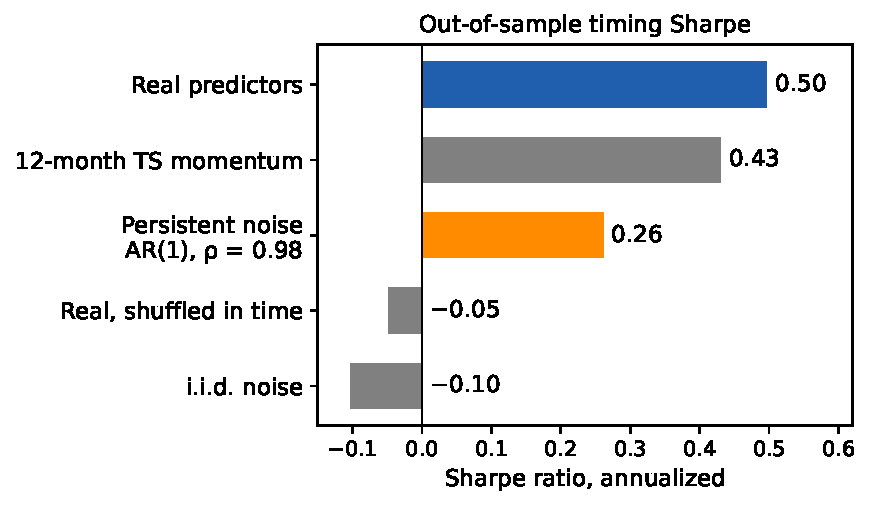
\includegraphics[width=\textwidth]{fig_placebo.pdf}\\
{\scriptsize RFF, $P=12{,}000$, $z=10^3$, $T=12$, $\gamma=2$, 1930--2020; noise: mean of 4--6 draws. Code: \texttt{critique\_checks.py}.}
\end{column}
\begin{column}{0.46\textwidth}
\footnotesize
\hl{Result.} Slow-moving pure noise earns $SR\approx0.26$, about half of the real result; i.i.d.\ or time-shuffled inputs earn $\le0$.\\
$\Rightarrow$ persistence $+$ 12-month window create momentum mechanically.\\
But real predictors keep alpha over 12-month TSMOM (IR 0.33, $t=3.1$).

\medskip
\hl{Holds up:} negative $R^2\neq$ no economic value; shrinkage is essential near $P\approx T$.

\smallskip
\hl{Contested:} that complexity itself creates predictability, and that the signal comes from the predictors rather than from momentum.

\smallskip
{\scriptsize Reply: Kelly \& Malamud (2025), ``Understanding the Virtue of Complexity''.}
\end{column}
\end{columns}
\end{frame}

\end{document}
